\documentclass[tikz,border=3pt]{standalone}

\usepackage{ctex}
\usepackage{tikz}
\usetikzlibrary{arrows.meta, calc, angles, quotes, positioning}

% TODO: 设置字体格式，与论文要求统一，提前缩放，引入时不进一步缩放
%\tikzset{
%	every node/.style={
%		font=\songti\fontsize{10.5pt}{12pt}\selectfont
%	}
%}

\begin{document}
	

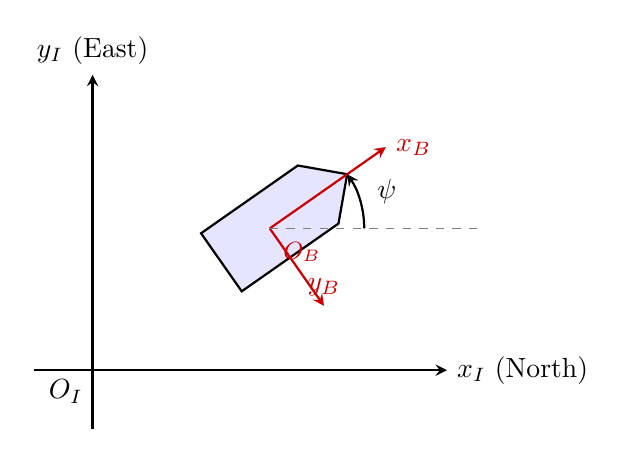
\begin{tikzpicture}[>=stealth, scale=1.5]
	
	% -------------------------------------------------------------------------
	% 1. 定义参数（方便调整尺寸）
	% -------------------------------------------------------------------------
	\def\L{1.6}   % 船全长
	\def\B{0.6}   % 船身宽
	\def\Bbow{0.2} % 船首尖端宽 (0表示全尖)
	\def\Lrect{1.0} % 矩形部分长度
	\def\psiAngle{35} % USV 的航向角
	
	% -------------------------------------------------------------------------
	% 2. 绘制大地坐标系 {I} (Earth-fixed Frame - NED)
	% -------------------------------------------------------------------------
%	\draw[->, thick, gray!80] (-0.5, 0) -- (3, 0) node[right, black] {$x_g$ (North)};
%	\draw[->, thick, gray!80] (0, -0.5) -- (0, 2.5) node[above, black] {$y_g$ (East)};
%	\node[below left, gray!80] at (0,0) {$O_g$};
	% -------------------------------------------------
	% 1. Global frame
	% -------------------------------------------------
	\coordinate (Og) at (0,0);
	\draw[->, thick] (-0.5, 0) -- (3, 0) node[right, black] {$x_I$ (North)};
	\draw[->, thick] (0, -0.5) -- (0, 2.5) node[above, black] {$y_I$ (East)};
	\node[below left] at (0,0) {$O_I$};
	% -------------------------------------------------------------------------
	% 3. 定义 USV 体轴坐标系 {B} 的原点 P(x, y)
	% -------------------------------------------------------------------------
	\coordinate (P) at (1.5, 1.2);
	\filldraw[black] (P) circle (1.5pt);
	
%	% 标注 P 点的大地坐标 (x, y)
%	\draw[dashed, gray!60] (P) -- (1.5, 0) node[below] {$x$};
%	\draw[dashed, gray!60] (P) -- (0, 1.2) node[left] {$y$};
%	\node[above left=2pt of P, font=\small] {$P(x,y)$};
	
	% -------------------------------------------------------------------------
	% 4. 绘制 USV 船体 (旋转角度 \psiAngle)
	% -------------------------------------------------------------------------
	\begin{scope}[shift={(P)}, rotate=\psiAngle]
		
		% 定义船体关键点 (相对于P点)
		\coordinate (SternL) at (-\Lrect/2, -\B/2);
		\coordinate (SternR) at (-\Lrect/2, \B/2);
		\coordinate (BowR)   at (\Lrect/2, \B/2);
		\coordinate (BowTip) at (\L/2, 0); % 船尖
		\coordinate (BowL)   at (\Lrect/2, -\B/2);
		
		% 绘制并填充船体 (流线型六边形)
		\draw[thick, fill=blue!10] 
		(SternL) -- (SternR) -- (BowR) -- (BowTip) -- (BowL) -- cycle;
		
		% 绘制质心标记 (CG) - 可选
		%\draw[fill=white] (0,0) circle (2pt);
		%\draw[fill=black] (0,0) -- ++(2pt,0) arc (0:90:2pt) -- cycle;
		%\draw[fill=black] (0,0) -- ++(-2pt,0) arc (180:270:2pt) -- cycle;
		
		% ---------------------------------------------------------------------
		% 5. 绘制体轴坐标系 {B} (Body-fixed Frame)
		% ---------------------------------------------------------------------
%		\draw[->, ultra thick, red!80!black] (0, 0) -- (1.2, 0) coordinate (Xb_axis) node[right] {$x_B$};
%		\draw[->, ultra thick, red!80!black] (0, 0) -- (0, -0.8) node[above] {$y_B$};
%		\node[below right=2pt of {(0,0)}, red!80!black, font=\small] {$O_B$};
		\draw[->, thick, red!80!black] (0, 0) -- (1.2, 0) coordinate (Xb_axis) node[right] {$x_B$};
		\draw[->, thick, red!80!black] (0, 0) -- (0, -0.8) node[above] {$y_B$};
		\node[below right=2pt of {(0,0)}, red!80!black, font=\small] {$O_B$};
		
		% ---------------------------------------------------------------------
		% 6. 标注运动学/动力学状态量 (Velocities & Rates)
		% ---------------------------------------------------------------------
		% Surge velocity u
%		\draw[->, thick, blue!80!black] (BowTip) -- ++(0.6, 0) node[right] {$u$};
%		
%		% Sway velocity v
%%		\draw[->, thick, blue!80!black] (0, \B/2) -- ++(0, -0.4) node[above] {$v$};
%		\draw[->, thick, blue!80!black] (0, 0) -- ++(0, -0.4) node[above] {$v$};
		
		% Yaw rate r (转头角速度)
		%			\draw[->, thick, orange!90!black] (0.3, 0) arc (0:220:0.3cm and 0.15cm);
%		\draw[<-, thick, orange!90!black] (0.3, 0) arc (0:220:0.3cm and 0.15cm);
%		\node[orange!90!black, font=\small] at (-0.3, 0.2) {$r$};
		
	\end{scope}
	
	% -------------------------------------------------------------------------
	% 7. 标注航向角 \psi (Heading Angle)
	% -------------------------------------------------------------------------
	% 绘制参考线（平行于 x_I）
	\draw[dashed, gray] (P) -- ++(1.8, 0) coordinate (Xref);
	
	% 使用 angles 库绘制角度
%	\pic [draw, ->, "$\psi$", angle eccentricity=1.3, angle radius=1.2cm, thick, green!50!black] 
%	{angle = Xref--P--Xb_axis};
	\pic [draw, ->, "$\psi$", angle eccentricity=1.3, angle radius=1.2cm, thick, black!50!black] 
	{angle = Xref--P--Xb_axis};
	
	% -------------------------------------------------------------------------
	% 8. 图例 (可选)
	% -------------------------------------------------------------------------
%	\node[draw, font=\footnotesize, align=left, fill=white, rounded corners] at (1.5, -0.8) {
%		$\{I\}$: Earth-fixed Frame (NED) \\
%		$\{B\}$: Body-fixed Frame \\
%		$[x, y, \psi]^T$: Position and heading \\
%		$[u, v, r]^T$: Velocities and yaw rate
%	};
	
\end{tikzpicture}
	
\end{document}